\documentclass[12pt]{article}

% language stuff
\usepackage{german}           % deutsche Überschriften etc.
\usepackage[utf8]{inputenc} % direkte Einbgabe von Umlauten

% Layout-Einstellungen
\usepackage{parskip}          % Abstand statt Einrückung
\frenchspacing                % no extra space after periods
\usepackage{parskip}          % paragraph gaps instead of indentation
\usepackage{times}            % default font Times
\tolerance=9000               % avoid words across right border

% miscellaneous
\usepackage{graphicx}         % graphics
\usepackage{hhline}           % double lines in tables
\usepackage{amsfonts}         % real numbers etc.
\usepackage[rightcaption]{sidecap} % figure captions on the right (optional)
\usepackage{hyperref}         % for URLs
\usepackage{listings}         % for code samples

% Hier bei Bedarf die Seitenränder einstellen
\usepackage{geometry}
%\geometry{a4paper}
\geometry{a4paper,left=25mm,right=25mm, top=3.0cm, bottom=3.0cm} 


%%%%%%%%%%%%%%%%%%%%%%%%%%%%%%%%%%%%%%%%%%%%%%%%%%%%%%%%%%%%%%
\title{\vspace*{-10mm}Hinweise zur Erstellung der Bachelorarbeit\\ mit \LaTeX}
\author{
% Autor und Email-Adresse ersetzen:
Christoph Dalitz\\
Hochschule Niederrhein\\
Fachbereich Elektrotechnik und Informatik\\
Reinarzstr. 49, 47805 Krefeld\\
{\tt christoph.dalitz{@}hsnr.de}
}
\date{20. Juni 2018}

%%%%%%%%%%%%%%%%%%%%%%%%%%%%%%%%%%%%%%%%%%%%%%%%%%%%%%%%%%%%%%
\begin{document}

\maketitle

%-------------------------------------------------------------
\begin{abstract}
%-------------------------------------------------------------
Ergänzend zum Latex-Template für eine Bachelorarbeit erläutert
dieses Dokument, wie die schriftliche Arbeit mit Latex erstellt
werden kann. Dabei wird insbesondere auf typische Fragen zum
Einbinden von Abbildungen und Code-Listings als Floating-Objekte
und zu den erforderlichen Angaben in der Literaturliste
eingegangen. Ferner enthält es meine persönlichen Empfehlungen
zum Schreibstil.
\end{abstract}

%-------------------------------------------------------------
% default a), b), c) numbering
\renewcommand{\labelenumi}{\alph{enumi})} 

%=============================================================


\section{Einführung}
%-------------------------------------------------------------
Zur Erstellung wissenschaftlicher Texte ist \LaTeX\ ein verbreitetes
Textsatzsystem. Um das Schreiben einer Abschlussarbeit zu erleichtern,
habe ich ein Template bereitgestellt, das als Startpunkt
für die eigene Abschlussarbeit genommen werden kann. Da jenes Template
nur das allgemeine Skelett einer realen Abschlussarbeit darstellt und
keine weiteren Informationen zum Arbeiten mit \LaTeX enthält, sind diese
Informationen in diesem Dokument zusammengefasst.

Die Arbeit ist im DIN A4-Format in zwei Exemplaren abzugeben:
\begin{itemize}
\item zwei gebundene Exemplare für die beiden Prüfer
\item ein {\em nicht} gebundenes Exemplar für den Hängeordner zur späteren
  Archivierung in der Bibliothek
\end{itemize}
Zusätzlich zur ausgedruckten schriftlichen Arbeit ist dem nicht gebundenen
Exemplar eine CD-ROM beizulegen,
die die Arbeit im PDF-Format enthält, ggf.~den im Rahmen der Arbeit 
entwickelten Sourcecode, sowie Abzüge zitierter Webseiten. Für weitere
allgemeine Informationen zur Bachelorarbeit sei auf das Merkblatt
des Fachbereichs hingewiesen, das von der Webseite des Fachbereichs
erhältlich ist.

Im Folgenden wird zunächst für \LaTeX-Anfänger beschrieben, wo es die
Software und Dokumentation zu \LaTeX\ gibt. Abschnitt \ref{sec:floats}
beschreibt das Einbinden von Grafiken und die Darstellung anderer ``Floating
Objects''. Der Abschnitt zu ``Inhalt und Stil'' gilt nur für Abschlussarbeiten,
bei denen ich Erstprüfer bin. Andere Dozenten haben ggf. andere Empfehlungen.
Der letzte Abschnitt \ref{sec:quellen} beschreibt, was bei den
Quellenangaben und Zitaten zu beachten ist.


\section{Software und Dokumentation}
%-------------------------------------------------------------
\LaTeX\ ist freie Software und ist bei allen Linux-Distributionen dabei.
Für Windows und MacOS X gibt es ebenfalls Distributionen. Einen Überblick
bietet Tabelle \ref{tbl:latexdists}.
%------------------------------------------------------------------------- 
\begin{table}[t]
\centering
\begin{tabular}{c|c|l}
{\em Distribution} & {\em Betriebssystem} & {\em URL} \\ \hline\hline
TexLive & Linux & bei Linux-Distribution dabei \\ \hline
MiKTeX & Windows &  \url{http://miktex.org/}\\ \hline
MacTeX & MacOS X & \url{http://www.tug.org/mactex/} \\ \hline
teTeX (Fink) & MacOS X & \url{http://www.finkproject.org/}
\end{tabular}
\caption{\label{tbl:latexdists} Überblick über gängige \LaTeX-Distributionen.
}
\end{table}
%------------------------------------------------------------------------- 

Den \LaTeX-Quellcode kann man mit einem beliebigen Texteditor erstellen und
bearbeiten, wobei viele Texteditoren Syntaxhighlighting für {\em *.tex} Dateien
eingebaut haben. Je nach Betriebssystem geeignete Editoren sind 
z.B.~unter Linux {\em gedit}, {\em kedit} oder {\em emacs},
unter Windows 
{\em Notepad++}\footnote{\url{http://notepad-plus.sourceforge.net/}}, und unter
MacOS X {\em TexShop}\footnote{\url{http://www.uoregon.edu/~koch/texshop/}}
oder {\em TextWrangler}\footnote{\url{http://www.barebones.com/products/TextWrangler/}}.
Mit der Anweisung
\begin{quote}
\verb+\usepackage[utf8]{inputenc}+
\end{quote}
im Vorspann können Umlaute direkt im Editor eingegeben werden, wobei das
Encoding {\em utf8} ggf.~durch das vom Editor verwendete Encoding
zu ersetzen ist.

Zum Nachschlagen von Befehlen und von Konzepten empfiehlt sich das
Zulegen eines Buches über \LaTeX. Die klassische deutschsprachige Referenz
ist das schon etwas ältere Buch von Kopka \cite{kopka91}, aber auch das
deutlich preiswertere Buch des Rechenzentrums Hannover (erhältlich
in unserer Hochschulbibliothek) ist eine gutes Handbuch \cite{rrzn06}.

\section{Floating Objects}
%-------------------------------------------------------------
\label{sec:floats}
Bitte vermeiden Sie die Unsitte, Abbildungen ohne erläuternde Unterschrift
(``Caption'') mitten in den Fließtext zu setzen! Grafiken, Tabellen und längere
Code-Listings sind als ``Floating Objects'' unabhängig vom Fließtext am Kopf
oder Fuß der Seite zu platzieren und mit einer selbsterklärenden kurzen
``Caption'' zu versehen.

Dafür gibt es in \LaTeX\ die Umgebungen {\em figure}, {\em table} und
{\em lstlisting} (aus dem Paket {\em listings}). Der Bezug auf das Objekt
erfolgt im Fließtext mit \verb+\ref+, das sich auf einen in der Caption
mit \verb+label+ gesetzten Anker bezieht. Ein Beispiel für eine solchen
Bezug auf eine {\em table} ist Tabelle \ref{tbl:latexdists}.

\subsection{Grafiken}
%-------------------------------------------------------------
Abbildungen im EPS oder PDF Format werden mit \verb+\includegraphics+
eingebunden. Als Floating-Umgebung ist {\em figure} zu verwenden. Ein Beispiel
finden Sie in Abb.~\ref{fig:grafik}. Wenn Sie bei schmalen Abbildungen
um Platz zu sparen die Caption seitlich statt unter der Grafik platzieren
wollen, können Sie statt {\em figure} die Umgebung {\em SCfigure}
aus dem Paket {\em sidecap} verwenden.

%------------------------------------------------------------------------- 
\begin{figure}[t]
\centering
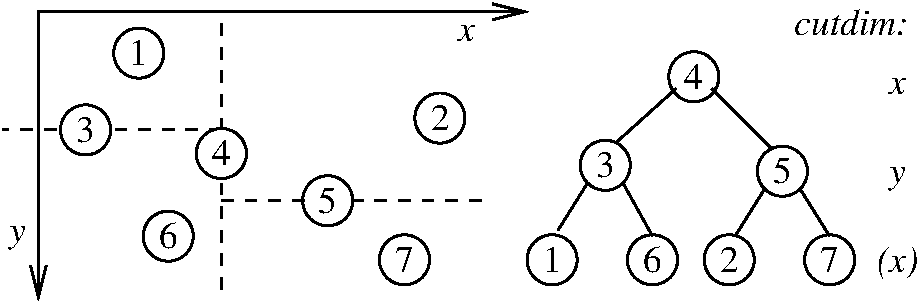
\includegraphics[scale=0.7]{grafik}
\caption{\label{fig:grafik} Beispiel für eine Abbildung (aus \cite{dalitz09}).
}
\end{figure}
%------------------------------------------------------------------------- 

Aus Qualitätsgründen sollten Sie für Strichzeichnungen mit Text unbedingt
Vektorgrafiken (EPS, PDF) und keine Rastergrafiken (PNG, JPEG) verwenden.
Die unterstützten Grafikformate hängen davon ab, ob Sie {\em pdflatex} 
(erzeugt direkt PDF) oder {\em latex} (erzeugt DVI, das mit {\em dvipdf}
nach PDF konvertiert wird) verwenden:
\begin{itemize}
\item {\em latex} unterstützt nur EPS
\item {\em pdflatex} unterstützt nur PNG oder PDF
\end{itemize}
Um aus einer EPS-Datei eine für {\em pdflatex} geeignete PDF-Datei zu erzeugen,
können Sie das Programm {\em epstopdf} verwenden, das Bestandteil der meisten
\LaTeX-Distributionen ist.

Um vom verwendeten latex-Kommando unabhängig zu sein, empfiehlt sich folgendes
Vorgehen:
\begin{itemize}
\item Erzeugen Sie die Grafik im EPS-Format, z.B.~{\em mygrafik.eps}
\item Wandeln Sie die Grafik mit {\em epstopdf} ins PDF-Format um, so dass
  Sie zwei Grafikdateien vorliegen haben: {\em mygrafik.eps} und 
  {\em mygrafik.pdf}
\item Binden Sie die Grafik beim {\em includegraphics}-Befehl ohne die
  Erweiterung ein, also
  \begin{quote}
    \verb+\includegraphics[scale=0.8]{mygrafik}+
  \end{quote}
  Dann wird sich der verwendete latex-Befehl die für ihn passende
  Grafikdatei aussuchen.
\end{itemize}

Zum Erstellen von Vektorgrafiken im EPS-Format können Sie z.B.~das Programm
{\em Xfig} verwenden \cite{xfig}, das bei Linux mitgeliefert wird und für
MacOS X
bei Fink\footnote{\url{http://www.finkproject.org/}} dabei ist. Dieses
Programm bietet auch die Möglichkeit, Rastergrafiken einzubinden und mit
Annotationen zu versehen. Weitere Alternativen sind die Programme
{\em Dia}\footnote{\url{http://live.gnome.org/Dia}} oder 
{\em Inkscape}\footnote{\url{http://www.inkscape.org/}}.

\subsection{Code-Listings}
%-------------------------------------------------------------
Kurze Code-Schnipsel können im Fließtext mit der {\em quote} Umgebung
dargestellt werden, z.B.
\begin{quote}
\begin{verbatim}
from gamera.kdtree import *
\end{verbatim}
\end{quote}
Längere Code-Ausschnitte sind wie Abbildungen zu behandeln und in einer
Floating-Umgebung unterzubringen. Dafür gibt es die Umgebung {\em lstlisting}
aus dem Paket {\em listings}, das auch eine Syntax-Hervorhebung hat.
Ein Beispiel für einen Sourcecode-Ausschnitt zeigt
Listing \ref{lst:sample}.

Insgesamt ist darauf zu achten, dass Code-Ausschnitte zugleich knapp und
informativ sind. Wenn Sie Sourcecode angeben, der über mehr als eine Seite
geht, machen Sie wahrscheinlich etwas falsch: weniger ist mehr.

%------------------------------------------------------------------------- 
\lstset{language=Python,
  basicstyle=\small \ttfamily,
  frame=bottomline,
  floatplacement=t!,
  aboveskip=0pt,
  captionpos=b
}
\begin{lstlisting}[float, caption={Beispiel für ein Code-Listing (aus \cite{dalitz09}).},
	label=lst:sample]
from gamera.kdtree import *

ccs = image.cc_analysis()
nodes = [KdNode([cc.center.x,cc.center.y], cc) for cc in ccs]
tree = KdTree(nodes)

nn_pairs = []
for cc in ccs:
   knn = tree.k_nearest_neighbors([cc.center.x,cc.center.y], 2)
   nn_pairs.append([cc, knn[1].data])
\end{lstlisting}
%------------------------------------------------------------------------- 

\section{Fremde Abbildungen, Fotos und Logos}
%-------------------------------------------------------------
Wenn Sie fremde Abbildungen oder Fotos verwenden wollen, müssen Sie
beachten, dass diese dem Urheberrechtsschutz unterliegen und somit die
in der Veranstaltung ``Rechtliche und gesellschaftliche Aspekte der
Informatik'' \cite{rga} gelernten Einschränkungen gelten.

Da die Bachelorarbeit eine wissenschaftliche Arbeit ist, können prinzipiell
auch fremde Bilder als Ganzes (``Großzitat'') unter Angabe der Quelle
wiedergegeben werden, allerdings nur, wenn dies der Erläuterung dient.

Das Einbinden von Markenzeichen (``Logos'') ist dagegen problematisch, zum
einen weil dies nicht zur Erläuterung sondern zur Dekoration dient,
zum anderen weil dadurch der Eindruck eines offiziellen Dokuments des
Markeninhabers entsteht.
Die Hochschule Niederrhein hat sogar die Verwendung
ihres Logos in Abschlussarbeiten untersagt\footnote{Laut einem Schreiben des damaligen Rektors, Hermann Ostendorf, vom 24.07.2007.}. Bitte verwenden
Sie deshalb grundsätzlich zu Dekorationszwecken {\em keine Logos}
in Ihrer Abschlussarbeit.

\section{Mathematische Gleichungen und Plots}
%-------------------------------------------------------------
Für mathematische Formeln gibt es die Umgebungen {\em displaymath} (ohne
Nummerierung) und {\em equation} (mit Nummerierung), z.B.
\begin{equation}
\label{eq:mean}
\overline{x} = \frac{1}{n}\sum_{i=1}^n x_i
\end{equation}
Auf Gleichung (\ref{eq:mean}) kann Bezug genommen werden mit {\em ref} und
{\em label}. Für mathematische Ausdrücke im Fließtext gibt es die \$...\$
Umgebung, z.B. $(x_1,x_2,\ldots,x_n)$.

Um Plots von Funktionsgraphen zu erzeugen, können Sie z.B. das Programm
{\em octave}\footnote{\url{http://www.octave.org}} verwenden, das Funktionsplots
u.a.~im FIG-Format speichern kann, so dass sie mit {\em xfig} \cite{xfig}
weiterbearbeitet werden können. Hier ein Beispiel für den Octave-Code zum
Zeichnen von Sinus und Kosinus in einem Plot und dessen Speichern im
FIG-Format:
\begin{quote}
\begin{verbatim}
x = 0:0.01:pi;
plot(x,sin(x));
hold on;
plot(x,cos(x));
print("plot.fig","-mono")
\end{verbatim}
\end{quote}
Zur grafischen Darstellung von Messwerten können Sie
{\em gnuplot}\footnote{\url{http://www.gnuplot.info/}} verwenden.
Wenn die Messdaten in der Datei {\em plot.dat} in der Form von durch
white Space getrennte $x$ und $y$ Werte (ein Paar pro Zeile) vorliegen,
können Sie wie folgt in gnuplot am Bildschirm dargestellt und in einer
Datei im EPS-Format gespeichert werden:
\begin{quote}
\begin{verbatim}
plot 'plot.dat' with lines title 'Messwerte'
set term postscript eps
set output 'plot.eps'
replot
\end{verbatim}
\end{quote}
Wenn Sie die Grafik noch nachbearbeiten wollen, können Sie statt des EPS-Formats
auch mit {\em set term fig} im FIG-Format speichern.

\section{Inhalt und Stil}
%-------------------------------------------------------------
Die Arbeit muss mit einer Einleitung beginnen, die einen Überblick über die
Themenstellung gibt und diese in einen größeren Kontext stellt. Am Ende
der Arbeit muss ein Fazit dessen was geleistet wurde und wie es weitergehen
kann.

Insgesamt muss aus der Arbeit hervorgehen, was von Ihnen durchgeführt wurde
und was durch Dritte vorgegeben war. Irgendwo geistert die Empfehlungen herum,
dass in Abschlussarbeiten das Wort ``ich'' zu vermeiden sei: 
{\em das ist Unsinn}!
Wenn Sie selber etwas getan haben, müssen Sie das Wort ``ich'' verwenden.
Beispiel:
\begin{verse}
{\em falsch:} Es wurde untersucht ...\\
{\em richtig:} Ich habe untersucht ...
\end{verse}
Die erste Formulierung bedeutetet, dass nicht Sie die Untersuchung
durchgeführt haben. Das kann ja sein, und dann müssen Sie das natürlich
auch so schreiben und für die fremde Untersuchung eine Quelle angeben.
Aber auch in diesem Fall sollten Sie schreiben, {\em wer} denn nun die
Untersuchung durchgeführt hat.


\section{Quellenangaben und Zitate}
%-------------------------------------------------------------
\label{sec:quellen}
Für Quellenangaben kann der in \LaTeX\ eingebaute Mechanismus 
({\em bibitem} und {\em cite}) verwendet
werden. Die Verwendung des Addons {\em BibTeX} ist für die in der Regel wenigen
Literaturangaben einer Bachelorarbeit eher Overkill. Für Zitate kann die
{\em quote} Umgebung verwendet werden, wobei immer anzugeben ist, woher
das Zitat stammt. So schreibt Sturm \cite{rrzn06}:
\begin{quote}
``\LaTeX\ bietet verschiedene Umgebungen an, um Text im Blocksatz, aber
trotzdem beidseitig eingerückt zu setzen.''
\end{quote}
Wenn Sie die Autoren von Quellen {\em im Fließtext} nennen, so gelten folgende
Regeln:
\begin{itemize}
\item bei bis zu zwei Autoren werden alle Autoren genannt
\item ab drei Autoren wird nur der erste Autor genannt und die anderen
  werden mit ``et al.'' (et alii = und andere) abgekürzt (in der zugehörigen
  Quellenangabe werden aber alle Autoren genannt, außer es sind sehr viele)
\end{itemize}
Bei Quellenangaben ist unbedingt darauf zu achten, dass {\em nur zitierfähige}
Quellen angegeben werden. Quellen, bei denen Sie den Autor oder das 
Publikationsjahr nicht ermitteln können (kann bei Webseiten problematisch
sein), können Sie nicht als Quellen angeben. Im Literaturverzeichnis sind
je nach Quellentyp folgende Angaben erforderlich:
\begin{description}
\item[Bücher:] Autor(en), Titel, Verlag, ggf.~Auflage, Jahr.
  Beispiele: \cite{kopka91} \cite{rrzn06}
\item[Zeitschriftenaufsätze:] Autor(en), Titel, Zeitschrift mit Bandangabe,
  Seitenangaben, Jahr. Beispiele: \cite{dalitz09} \cite{dalitz08}
\item[Webseiten:] Autor(en), Titel, URL, Jahr der Publikation ({\em nicht}
  des Abrufs: bei einem Buch geben Sie ja auch nicht den Zeitpunkt des Lesens
  an!). Beispiel: \cite{website}
\item[Software:] Autor(en) oder Hersteller, Name, Version, Jahr, bei
  OpenSource Software ggf.~URL. Beispiel: \cite{xfig}
\end{description}
Aufgrund der fehlenden Überprüfbarkeit sind Webseiten als Quellenangaben
außer als Bezugsquellen für OpenSource-Software oft problematisch.
Deshalb sind auf
der der Bachelorarbeit beizulegenden CD-ROM auch Kopien zitierter
Webseiten zu speichern. Eine Möglichkeit
bei nicht zitierfähigen Quellen besteht evtl.~darin, sie als Fußnoten
anzugeben.

Ein wichtiger Hinweis noch zu Wikipedia\footnote{http://wikipedia.org/}:
Wikipedia ist keine Primärquelle, sondern ein Lexikon. Im allgemeinen ist
Wikipedia nicht zitierfähig, es ist aber trotzdem eine nützliche Ressource:
wie bei einem Lexikon liefert es einen ersten Überblick und die Quellenangaben
am Fuß der Seite führen manchmal zu zitierfähigen Quellen. Aber die dort
angegebenen Quellen müssen Sie natürlich erst noch sichten und auf Ihren
Wert hin untersuchen! M.a.W.: Wikipedia kann als Startpunkt einer Recherche
nützlich sein, ist jedoch nicht Endergebnis einer Recherche!

% Literaturverzeichnis
%-------------------------------------------------------------
%\newpage
\begin{thebibliography}{9}
\raggedright
\bibitem{kopka91} H.~Kopka: {\em LaTeX Bd.~1: Einführung.}
  Pearson Studium, 5.~Aufl.~(2005)
\bibitem{rrzn06} T.F.~Sturm: {\em Einführung in das LATEX Textsatzsystem.}
  RRZN der Universität Hannover, 1.~Aufl.~(2006)
\bibitem{dalitz09} C.~Dalitz: {\em Kd-Trees for Document Layout Analysis.}
  In C.~Dalitz (Ed.): ``Document Image Analysis with the Gamera Framework.''
  Schriftenreihe des Fachbereichs Elektrotechnik und Informatik,
  Hochschule Niederrhein, vol. 8, pp. 39-52, Shaker Verlag (2009) 
\bibitem{dalitz08} C.~Dalitz, M.~Droettboom, B.~Pranzas, I.~Fujinaga:
  {\em A Comparative Study of Staff Removal Algorithms.}
  IEEE Transactions on Pattern Analysis and Machine Intelligence, vol. 30,
  pp. 753-766 (2008)
\bibitem{website} M.~Droettboom, C.~Dalitz: {\em The Gamera Homepage.}
  \url{http://gamera.sourceforge.net/} (2008-2010)
\bibitem{xfig} B.V.~Smith et al.: 
  {\em Xfig Drawing Program for the X Windows System.} Version 3.2.5 (2009)
  (siehe \url{http://www.xfig.org/})
\bibitem{rga} C.~Dalitz: {\em Rechtliche und gesellschaftliche Aspekte der
  Informatik.} Lehrveranstaltung an der Hochschule Niederrhein im Studiengang
  ``Bachelor Informatik'', Wintersemester 2009/10
\end{thebibliography}


\end{document}

